%  \documentclass[oneside,11pt]{article}

% \input{preamble.tex}
% %%% HELPER CODE FOR DEALING WITH EXTERNAL REFERENCES
% \usepackage{xr}
% \makeatletter
% \newcommand*{\addFileDependency}[1]{
%   \typeout{(#1)}
%   \@addtofilelist{#1}
%   \IfFileExists{#1}{}{\typeout{No file #1.}}
% }
% \makeatother


% \newcommand*{\myexternaldocument}[1]{
%     \externaldocument{#1}
%     \addFileDependency{#1.tex}
%     \addFileDependency{#1.aux}
% }

% %\myexternaldocument{OA}

% %%%%%%%%%%%%%%%%%%%%%%%%%%%%%%%% DOCUMENT
% \begin{document}

%%%%%%%%%%%%%%%%%%%%%%%%%%%%%%%%%%%%%%%%%%%%%%%

% APPENDIX 
\setcounter{table}{0}
\setcounter{figure}{0}
\setcounter{section}{0}
\pagenumbering{gobble}


\begin{center}
	\LARGE Bargaining with (more) common priors in the field \\[0.5em]
	\Large{Appendix $-$ For Online Publication} \\[1em]
	\large \author{Joyce Sadka \and Enrique Seira  \and Christopher Woodruff}
\end{center}

\appendix
\pagenumbering{arabic}
\renewcommand\thefigure{OA-\arabic{figure}}
\renewcommand\thetable{OA-\arabic{table}}
\renewcommand*{\thepage}{OA - \arabic{page}}
\renewcommand\thesection{Appendix \Alph{section}.}
\renewcommand\thesubsection{\Alph{section}.\arabic{subsection}}

%\renewcommand{\cftparskip}{0em} % NOT NEEDED
\renewcommand\cftsecdotsep{\cftdotsep}
\renewcommand\cftsubsecdotsep{\cftnodots}
\renewcommand{\cftsecnumwidth}{6em}
 \renewcommand{\cftpnumalign}{r}
%\renewcommand{\cftsecleader}{\normalfont\cftdotfill{\cftsecdotsep}}


\renewcommand{\cftsecleader}{\cftdotfill{\cftsecdotsep}\hspace{1.8em}}
%\renewcommand{\cftsecpagefont}{20em}
%\renewcommand{\cftfignumwidth}{6em}
%\renewcommand{\cfttabnumwidth}{3.3em}

%\tableofcontents
\etocdepthtag.toc{mtappendix}
\etocsettagdepth{mtchapter}{none}
\etocsettagdepth{mtappendix}{subsection}

\setstretch{0.9}
%\renewcommand\contentsname{} % the empty name

\begingroup
\let\clearpage\relax
%\vspace{-1.5em} % the removed space. Set as appropriate
\tableofcontents
\endgroup


\newpage

\section{ -Balance in covariates}
\vspace{.2in}

\begin{figure}[H]
     \caption{RD plots (Calculator treatment; running variable : Tenure)}
    \label{rd_covs_tenure_t2}
\begin{center}
\begin{subfigure}{0.31\textwidth}
\caption{Anger}
        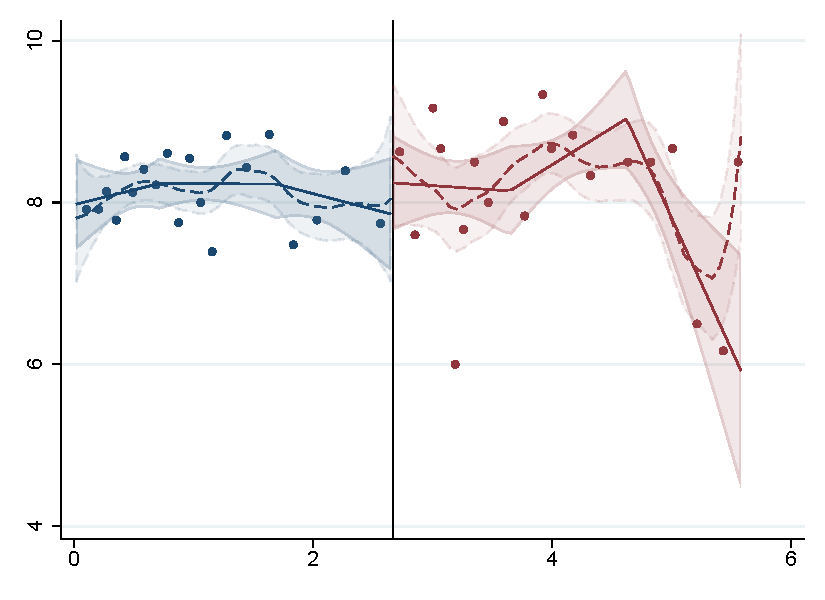
\includegraphics[width=\textwidth]{Figuras/rdplot_nivel_de_felicidad_tenure_2.pdf}
    \end{subfigure}
    \begin{subfigure}{0.31\textwidth}
\caption{More than High-School}
        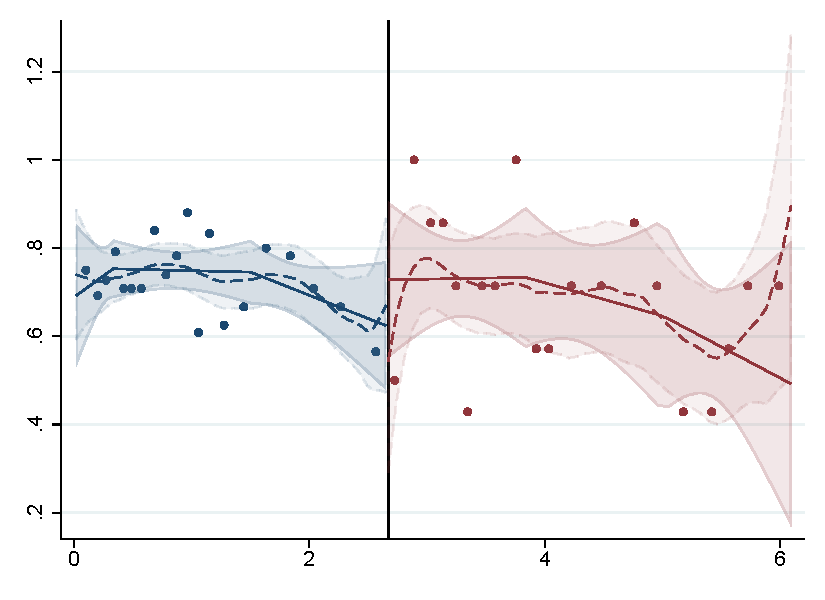
\includegraphics[width=\textwidth]{Figuras/rdplot_high_school_tenure_2.pdf}
    \end{subfigure}
\begin{subfigure}{0.31\textwidth}
\caption{Recruitment}
        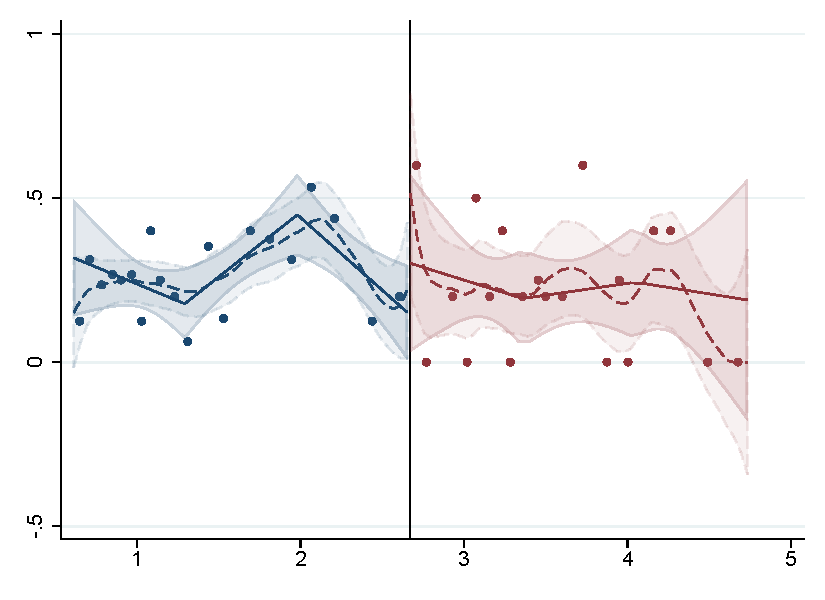
\includegraphics[width=\textwidth]{Figuras/rdplot_reclutamiento_tenure_2.pdf}
    \end{subfigure}
    \begin{subfigure}{0.31\textwidth}
\caption{At will worker}
        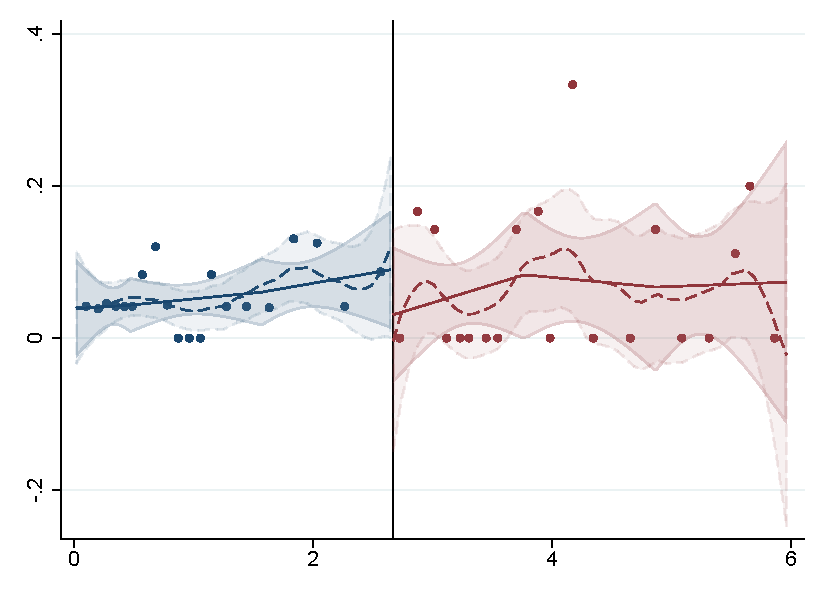
\includegraphics[width=\textwidth]{Figuras/rdplot_dummy_confianza_tenure_2.pdf}
    \end{subfigure}        
    \begin{subfigure}{0.31\textwidth}
\caption{Weekly hours}
        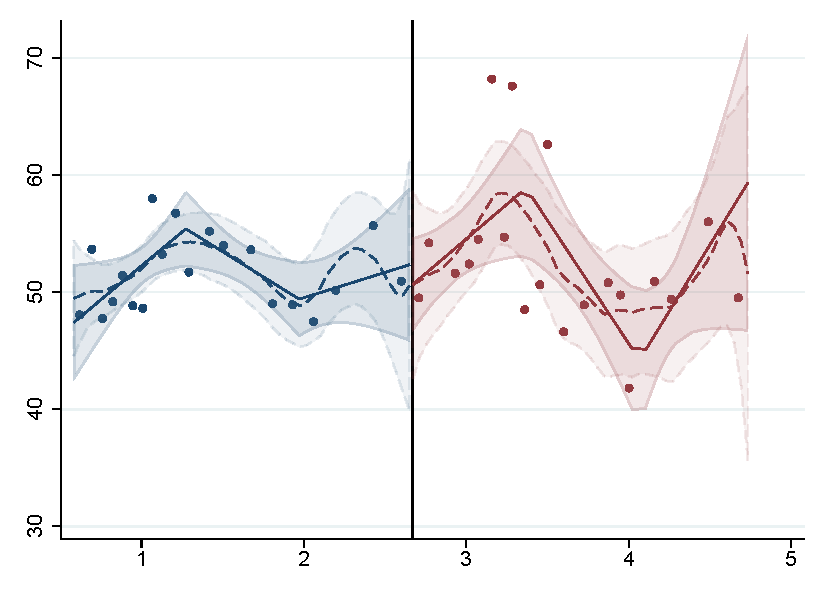
\includegraphics[width=\textwidth]{Figuras/rdplot_horas_sem_tenure_2.pdf}
    \end{subfigure}    
    \begin{subfigure}{0.31\textwidth}
\caption{Informal worker}
        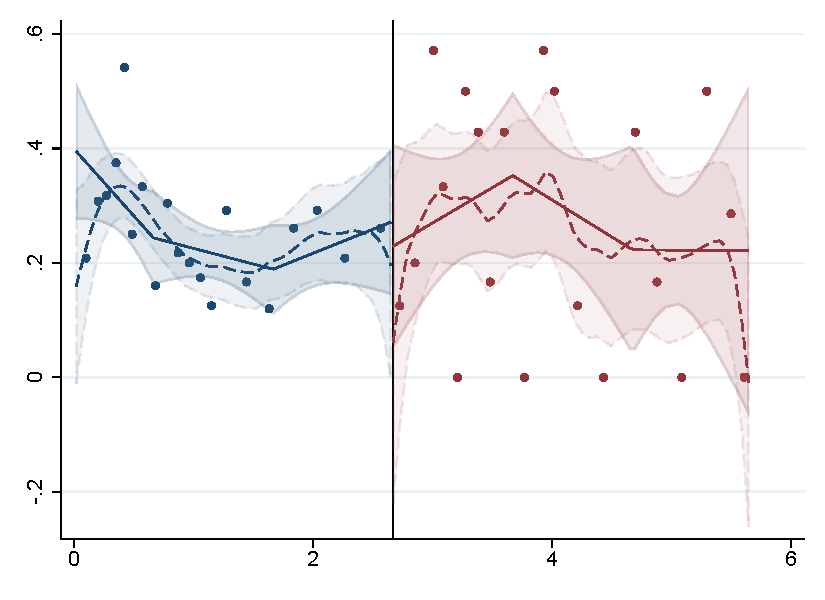
\includegraphics[width=\textwidth]{Figuras/rdplot_dummy_sarimssinfo_tenure_2.pdf}
    \end{subfigure}       
\begin{subfigure}{0.31\textwidth}
\caption{Legal entitlement}
        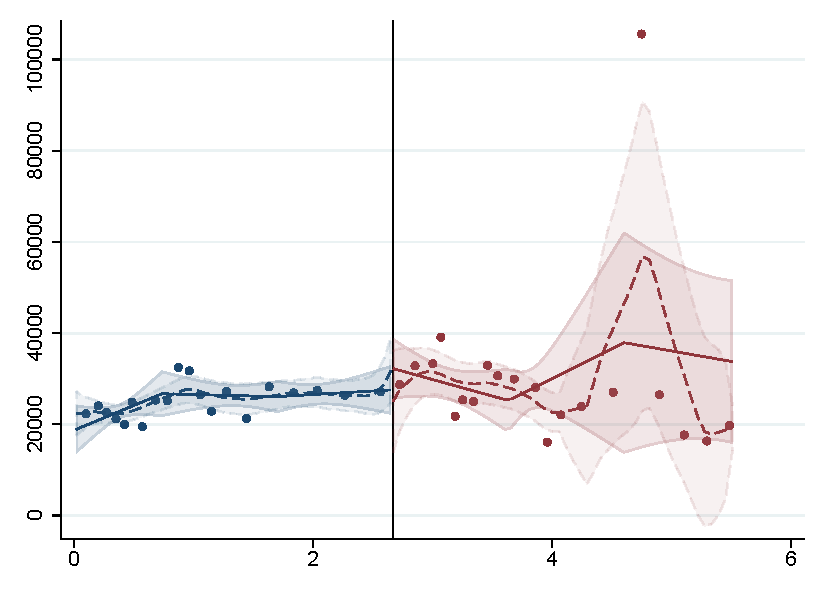
\includegraphics[width=\textwidth]{Figuras/rdplot_c_min_indem_tenure_2.pdf}
    \end{subfigure}
    \begin{subfigure}{0.31\textwidth}
\caption{Total entitlement}
        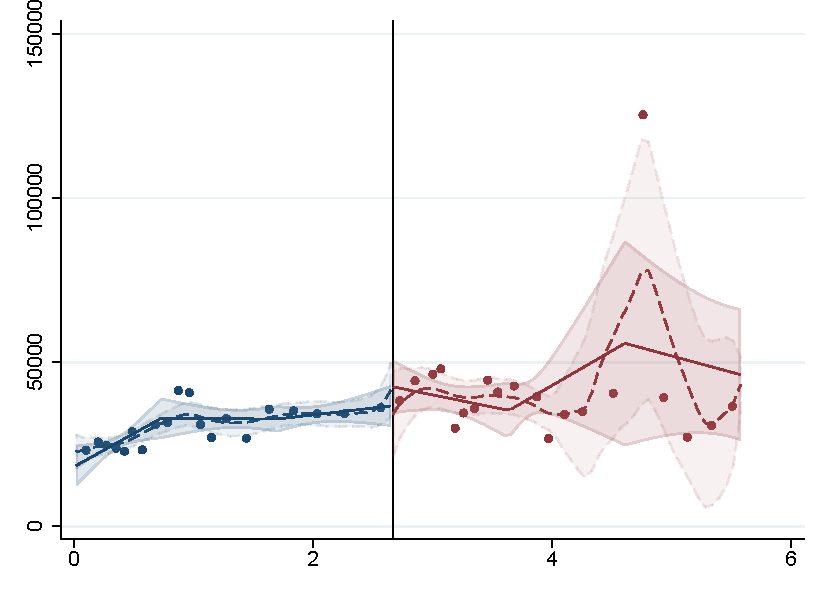
\includegraphics[width=\textwidth]{Figuras/rdplot_c_min_total_tenure_2.pdf}
    \end{subfigure}        
\begin{subfigure}{0.31\textwidth}
\caption{Woman}
        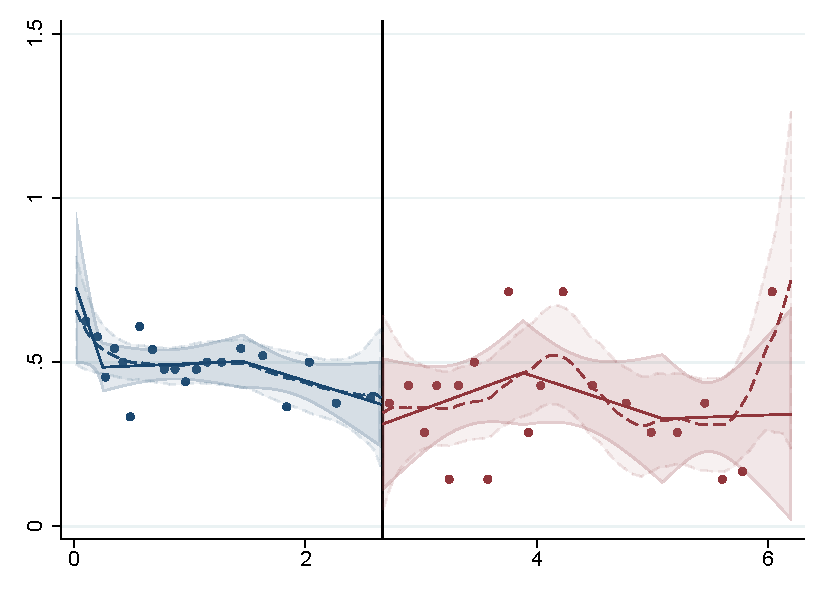
\includegraphics[width=\textwidth]{Figuras/rdplot_mujer_tenure_2.pdf}
    \end{subfigure}
  \end{center}
  
    \scriptsize Regression discontinuity plots using 1) local polynomial smoothing 2) B-splines. \textcolor{yellow}{Me falta ajustar cosas de inferencia cuando uso los splines.}
%\textit{Scripts: }  \texttt{plot\_rd\_covs.do}
\end{figure}




\begin{figure}[H]
     \caption{RD plots (Calculator treatment; running variable : Daily wage)}
    \label{rd_covs_dw_t2}
\begin{center}
\begin{subfigure}{0.31\textwidth}
\caption{Anger}
        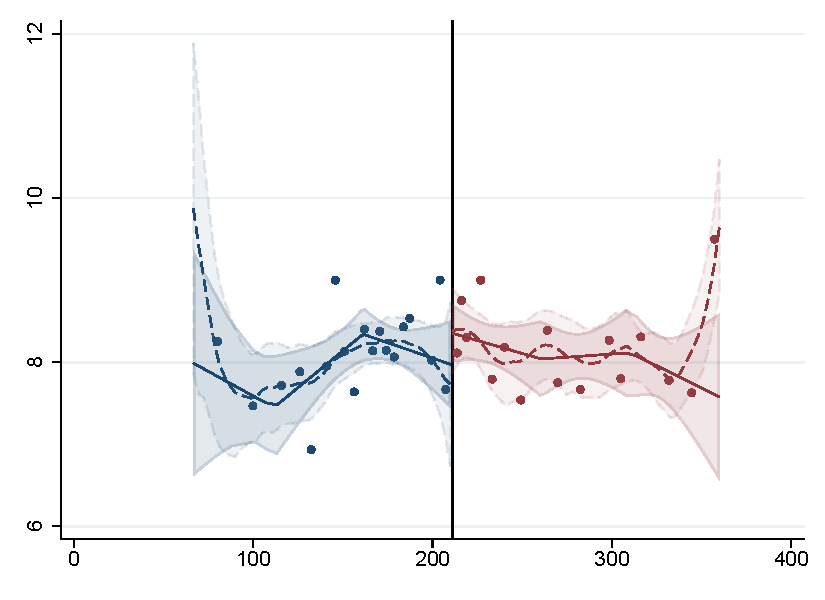
\includegraphics[width=\textwidth]{Figuras/rdplot_nivel_de_felicidad_dw_2.pdf}
    \end{subfigure}
    \begin{subfigure}{0.31\textwidth}
\caption{More than High-School}
        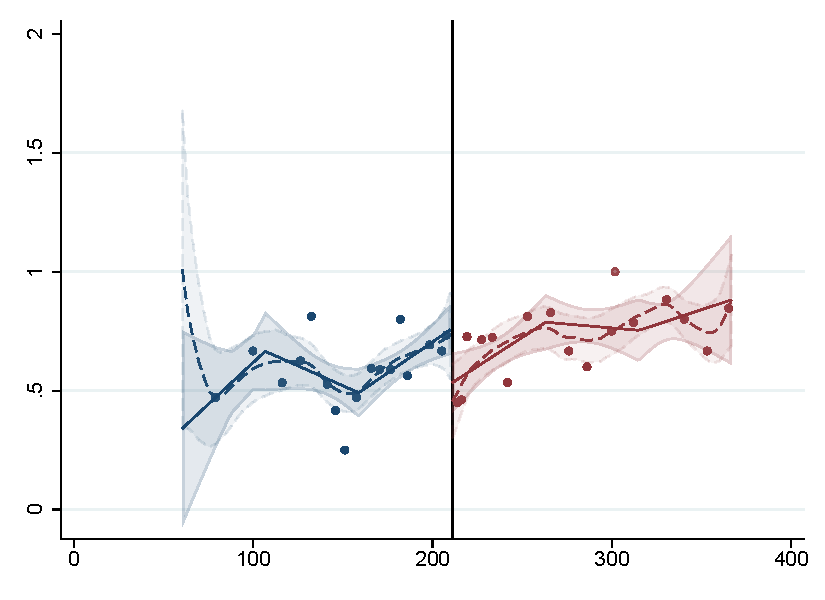
\includegraphics[width=\textwidth]{Figuras/rdplot_high_school_dw_2.pdf}
    \end{subfigure}
\begin{subfigure}{0.31\textwidth}
\caption{Recruitment}
        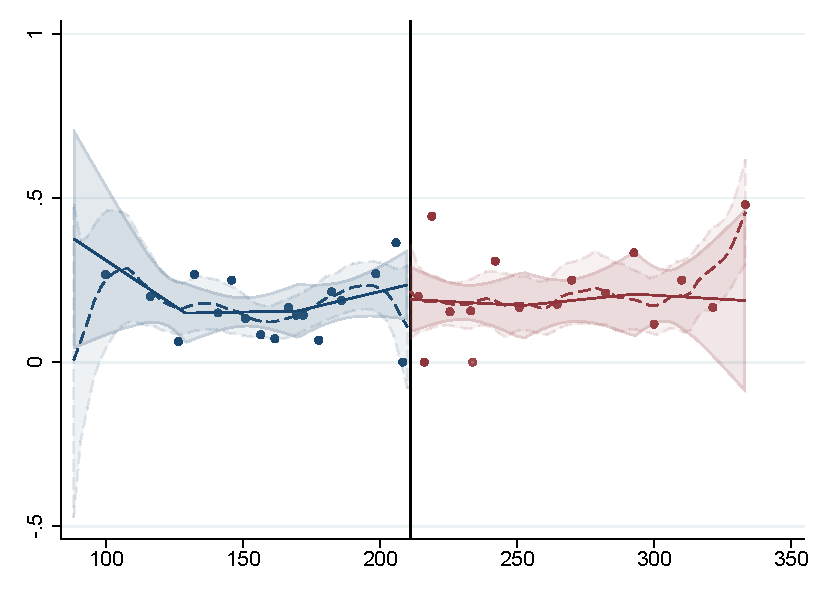
\includegraphics[width=\textwidth]{Figuras/rdplot_reclutamiento_dw_2.pdf}
    \end{subfigure}
    \begin{subfigure}{0.31\textwidth}
\caption{At will worker}
        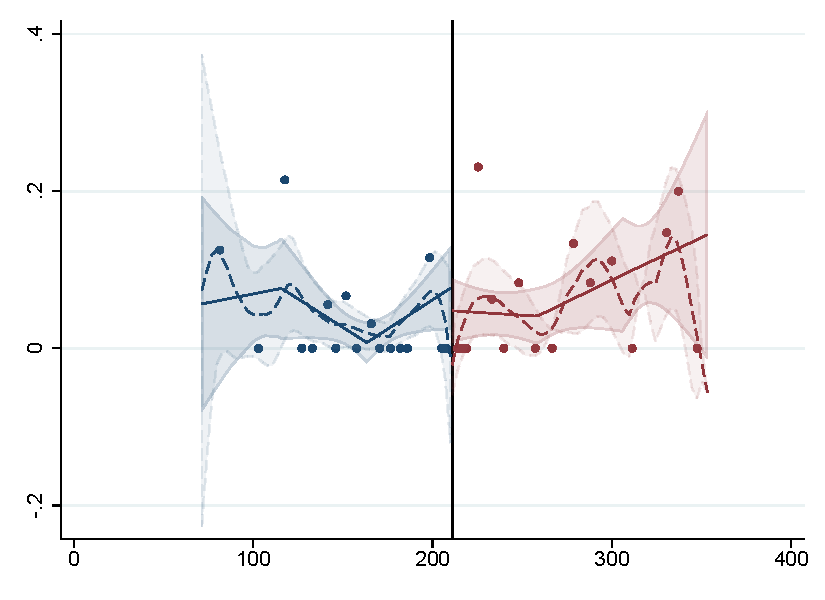
\includegraphics[width=\textwidth]{Figuras/rdplot_dummy_confianza_dw_2.pdf}
    \end{subfigure}        
    \begin{subfigure}{0.31\textwidth}
\caption{Weekly hours}
        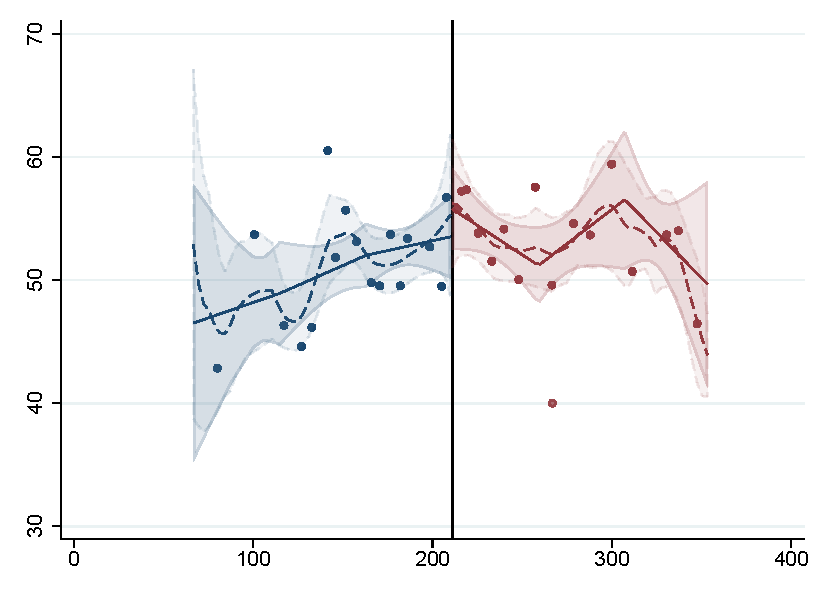
\includegraphics[width=\textwidth]{Figuras/rdplot_horas_sem_dw_2.pdf}
    \end{subfigure}    
    \begin{subfigure}{0.31\textwidth}
\caption{Informal worker}
        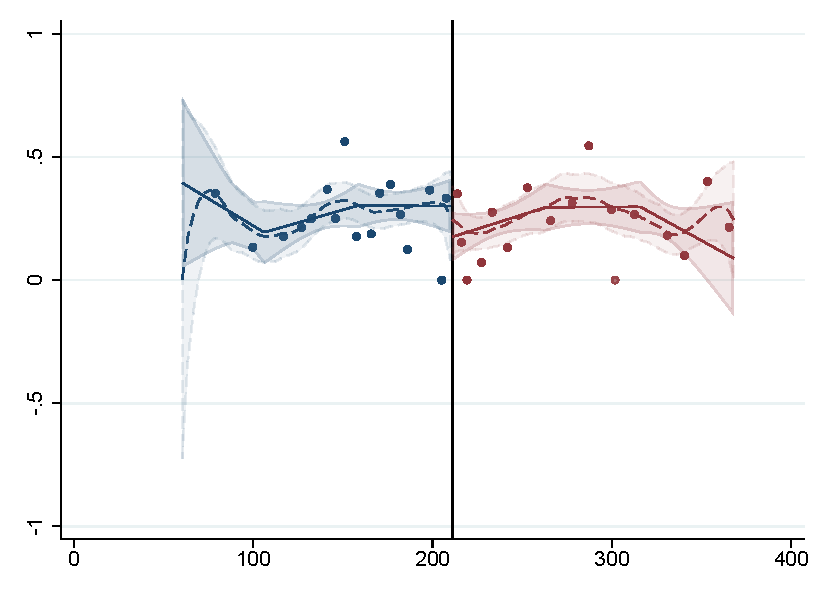
\includegraphics[width=\textwidth]{Figuras/rdplot_dummy_sarimssinfo_dw_2.pdf}
    \end{subfigure}       
\begin{subfigure}{0.31\textwidth}
\caption{Legal entitlement}
        \includegraphics[width=\textwidth]{Figuras/rdplot_c_min_indem_dw_2.pdf}
    \end{subfigure}
    \begin{subfigure}{0.31\textwidth}
\caption{Total entitlement}
        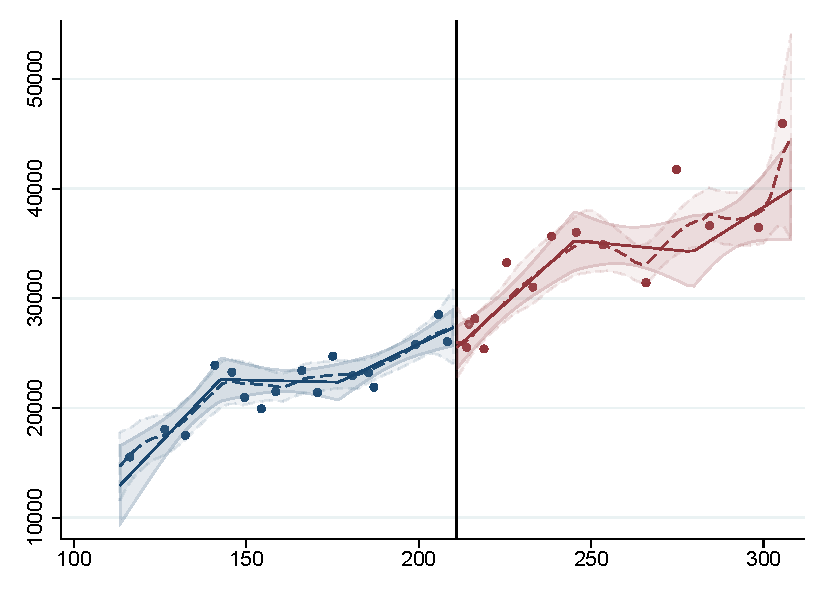
\includegraphics[width=\textwidth]{Figuras/rdplot_c_min_total_dw_2.pdf}
    \end{subfigure}        
\begin{subfigure}{0.31\textwidth}
\caption{Woman}
        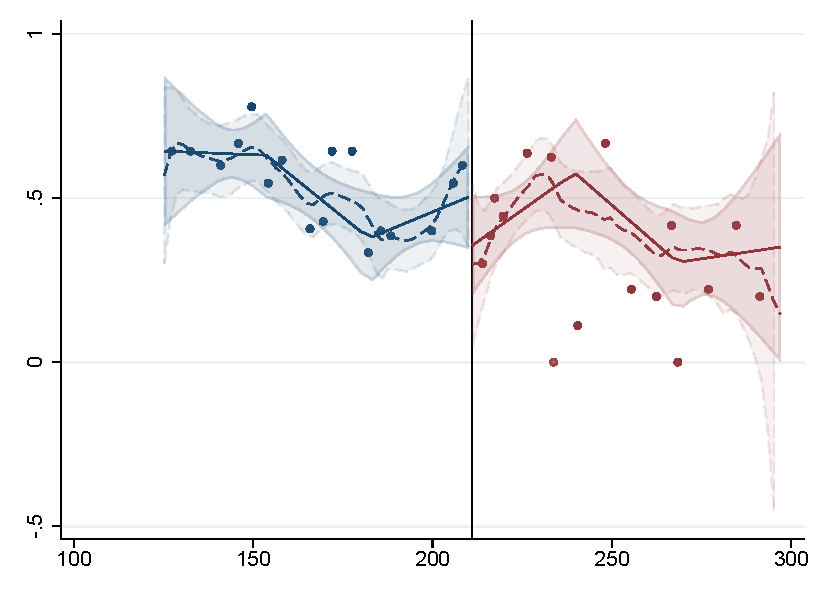
\includegraphics[width=\textwidth]{Figuras/rdplot_mujer_dw_2.pdf}
    \end{subfigure}
  \end{center}
  
    \scriptsize Regression discontinuity plots using 1) local polynomial smoothing 2) B-splines. \textcolor{yellow}{Me falta ajustar cosas de inferencia cuando uso los splines.}
%\textit{Scripts: }  \texttt{plot\_rd\_covs.do}
\end{figure}

\begin{figure}[H]
     \caption{RD plots (Calculator treatment; running variable : Tenure \& Daily wage)}
    \label{rd_covs_2_4_t2}
\begin{center}
\begin{subfigure}{0.31\textwidth}
\caption{Anger}
        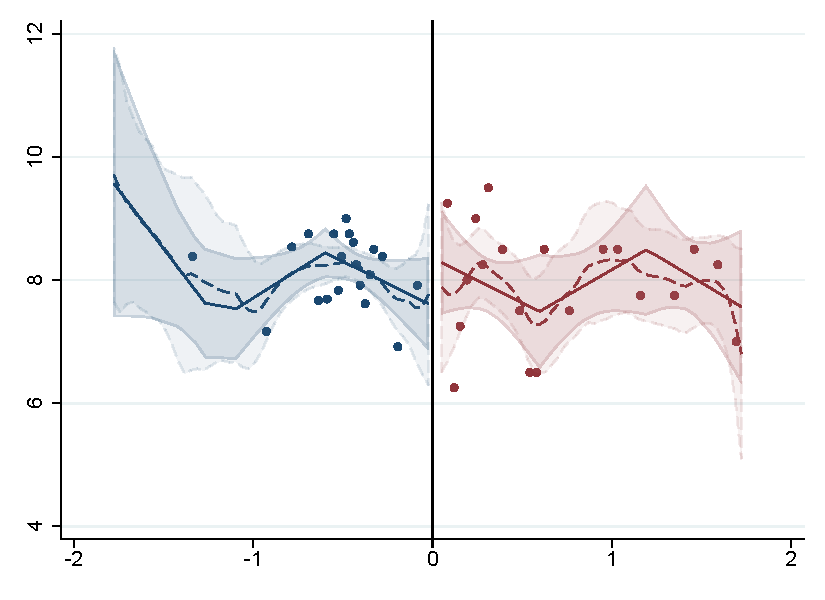
\includegraphics[width=\textwidth]{Figuras/rdplot_nivel_de_felicidad_2_4_2.pdf}
    \end{subfigure}
    \begin{subfigure}{0.31\textwidth}
\caption{More than High-School}
        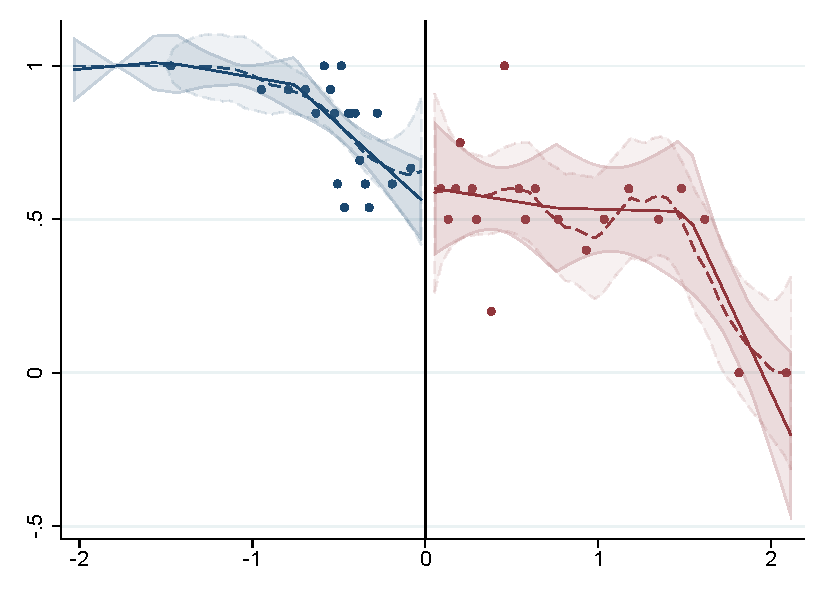
\includegraphics[width=\textwidth]{Figuras/rdplot_high_school_2_4_2.pdf}
    \end{subfigure}
\begin{subfigure}{0.31\textwidth}
\caption{Recruitment}
        \includegraphics[width=\textwidth]{Figuras/rdplot_reclutamiento_2_4_2.pdf}
    \end{subfigure}
    \begin{subfigure}{0.31\textwidth}
\caption{At will worker}
        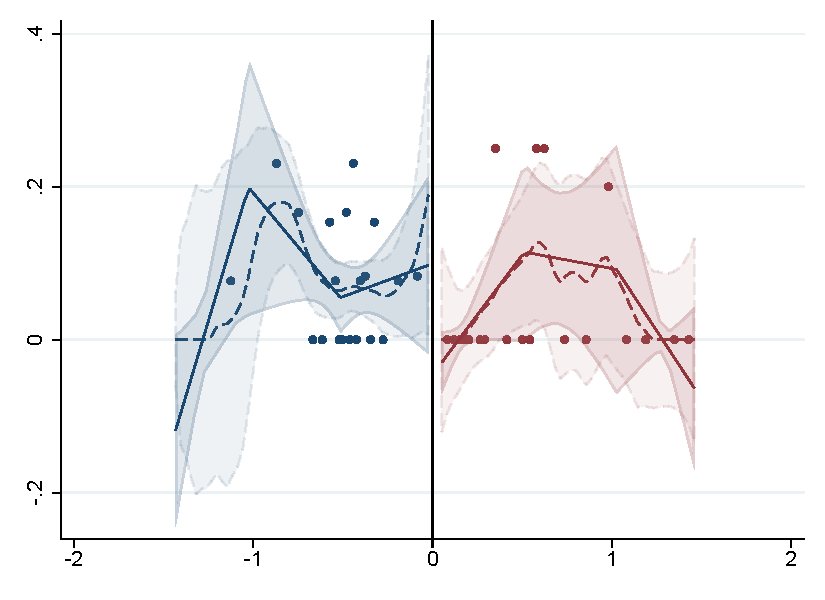
\includegraphics[width=\textwidth]{Figuras/rdplot_dummy_confianza_2_4_2.pdf}
    \end{subfigure}        
    \begin{subfigure}{0.31\textwidth}
\caption{Weekly hours}
        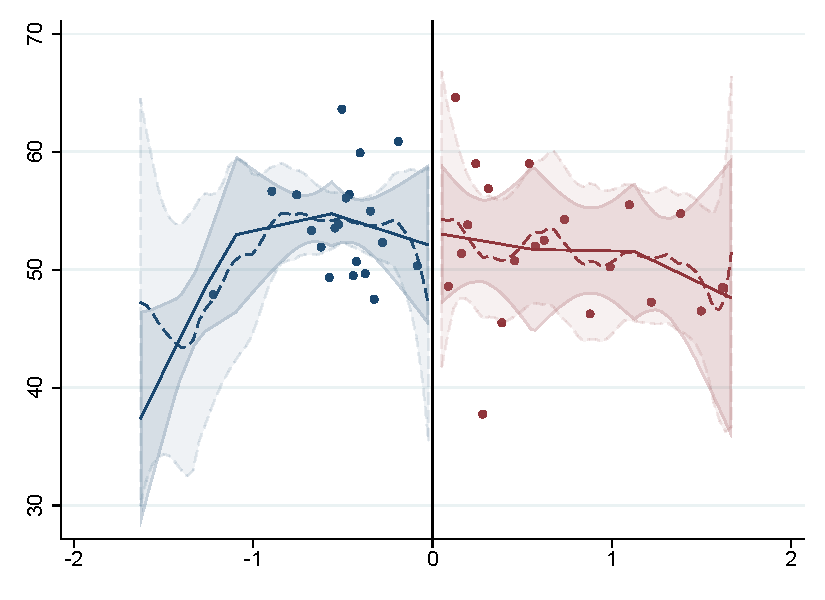
\includegraphics[width=\textwidth]{Figuras/rdplot_horas_sem_2_4_2.pdf}
    \end{subfigure}    
    \begin{subfigure}{0.31\textwidth}
\caption{Informal worker}
        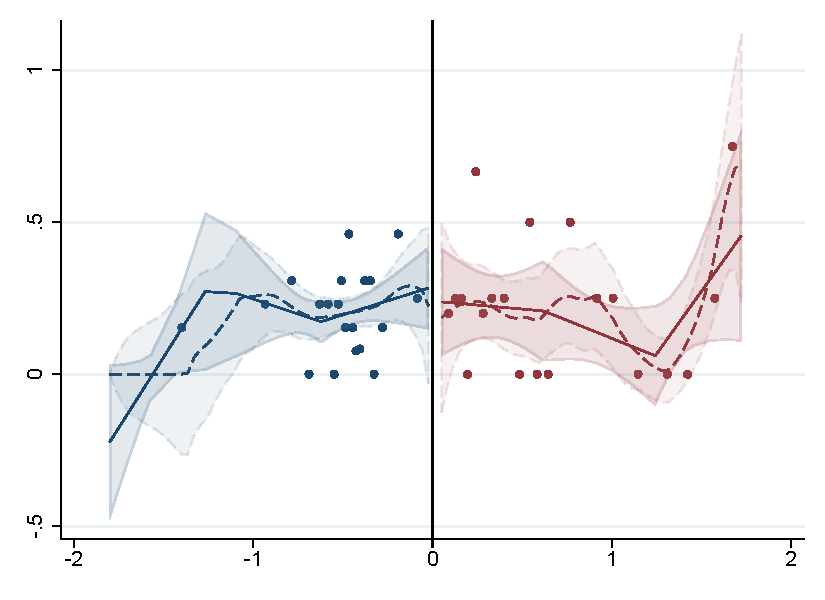
\includegraphics[width=\textwidth]{Figuras/rdplot_dummy_sarimssinfo_2_4_2.pdf}
    \end{subfigure}       
\begin{subfigure}{0.31\textwidth}
\caption{Legal entitlement}
        \includegraphics[width=\textwidth]{Figuras/rdplot_c_min_indem_2_4_2.pdf}
    \end{subfigure}
    \begin{subfigure}{0.31\textwidth}
\caption{Total entitlement}
        \includegraphics[width=\textwidth]{Figuras/rdplot_c_min_total_2_4_2.pdf}
    \end{subfigure}        
\begin{subfigure}{0.31\textwidth}
\caption{Woman}
        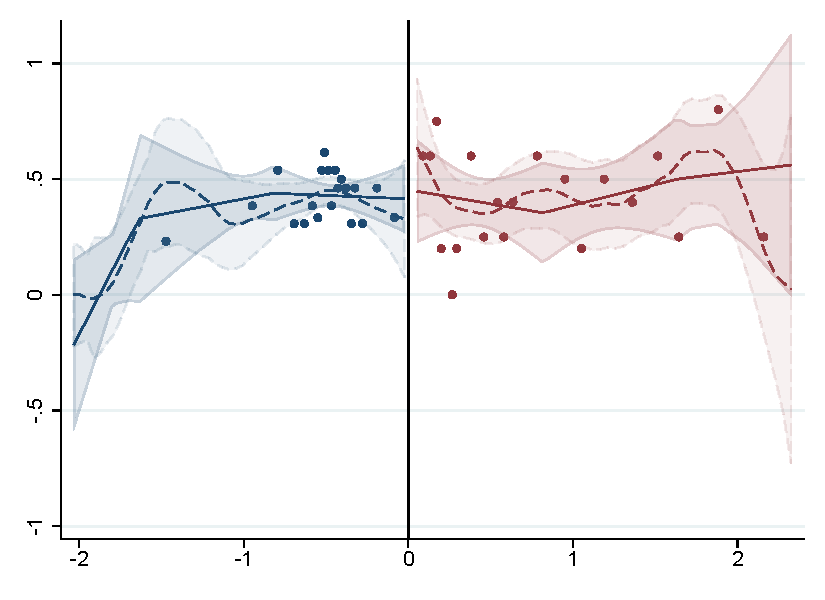
\includegraphics[width=\textwidth]{Figuras/rdplot_mujer_2_4_2.pdf}
    \end{subfigure}
  \end{center}
  
    \scriptsize Regression discontinuity plots using 1) local polynomial smoothing 2) B-splines. \textcolor{yellow}{Me falta ajustar cosas de inferencia cuando uso los splines.}
%\textit{Scripts: }  \texttt{plot\_rd\_covs.do}
\end{figure}


%__________________________________________________________________________
%__________________________________________________________________________
%__________________________________________________________________________
%__________________________________________________________________________

\section{ -Robustness : Validation and falsification of the RD design}
\vspace{.2in}


\begin{figure}[H]
     \caption{RD plots (Control)}
    \label{rd_t1}
\begin{center}
\begin{subfigure}{0.31\textwidth}

\caption{Tenure}
        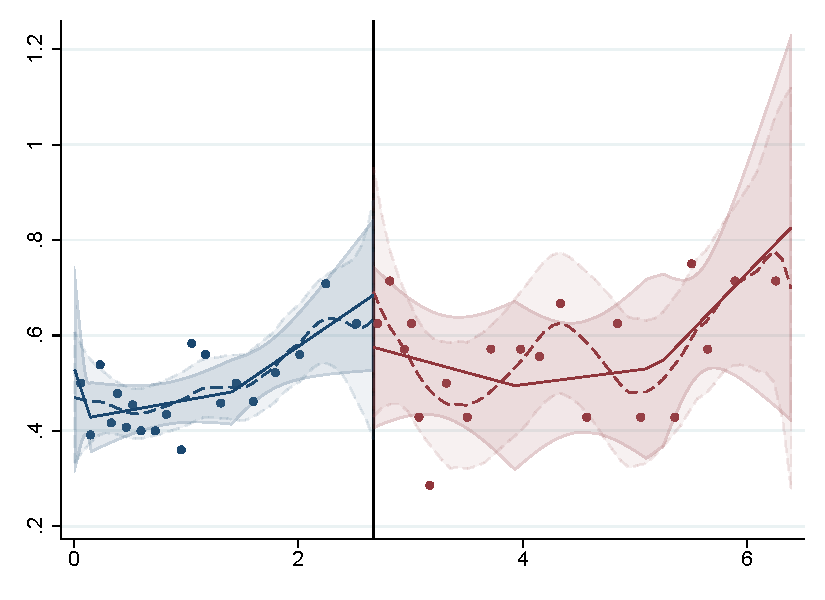
\includegraphics[width=\textwidth]{Figuras/rdplot_conflicto_arreglado_tenure_1.pdf}
    \end{subfigure}
    \begin{subfigure}{0.31\textwidth}
\caption{Daily wage}
        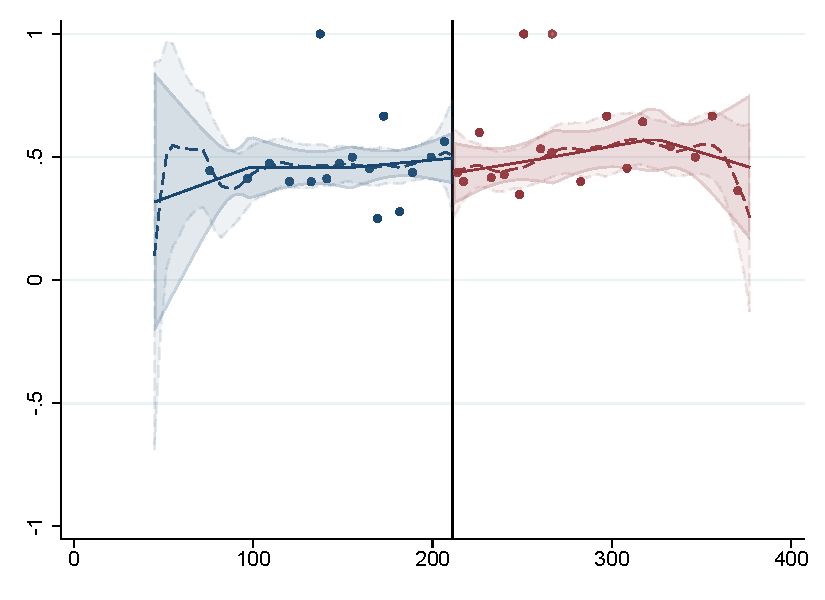
\includegraphics[width=\textwidth]{Figuras/rdplot_conflicto_arreglado_dw_1.pdf}
    \end{subfigure}        
    \begin{subfigure}{0.31\textwidth}
\caption{Tenure \& Daily wage}
        \includegraphics[width=\textwidth]{Figuras/rdplot_conflicto_arreglado_2_4_1.pdf}
    \end{subfigure}
  \end{center}
  
    \scriptsize Regression discontinuity plots using 1) local polynomial smoothing 2) B-splines. \textcolor{yellow}{Me falta ajustar cosas de inferencia cuando uso los splines.}
%\textit{Scripts: }  \texttt{plot\_rd\_control.do}
\end{figure}



%__________________________________________________________________________
%__________________________________________________________________________
%__________________________________________________________________________
%__________________________________________________________________________

\begin{figure}[H]
     \caption{Estimation for artificial cutoffs (Calculator treatment)}
    \label{placebo_cutoff_t2}
\begin{center}
\begin{subfigure}{0.475\textwidth}
\caption{Tenure}
        \includegraphics[width=\textwidth]{Figuras/placebo_cut_tenure_2.pdf}
    \end{subfigure}
    \begin{subfigure}{0.475\textwidth}
\caption{Daily wage}
        \includegraphics[width=\textwidth]{Figuras/placebo_cut_dw_2.pdf}
    \end{subfigure}
  \end{center}
  
    \scriptsize 
%\textit{Scripts: }  \texttt{placebo\_cutoff.do}
\end{figure}


\begin{figure}[H]
     \caption{Estimation for artificial cutoffs (Calculator + letter treatment)}
    \label{placebo_cutoff_t3}
\begin{center}
\begin{subfigure}{0.475\textwidth}
\caption{Tenure}
        \includegraphics[width=\textwidth]{Figuras/placebo_cut_tenure_3.pdf}
    \end{subfigure}
    \begin{subfigure}{0.475\textwidth}
\caption{Daily wage}
        \includegraphics[width=\textwidth]{Figuras/placebo_cut_dw_3.pdf}
    \end{subfigure}
  \end{center}
  
    \scriptsize 
%\textit{Scripts: }  \texttt{placebo\_cutoff.do}
\end{figure}



%__________________________________________________________________________
%__________________________________________________________________________
%__________________________________________________________________________
%__________________________________________________________________________

\begin{figure}[H]
     \caption{Donut-hole sensitivity (Calculator treatment)}
    \label{donut_hole_t2}
\begin{center}
\begin{subfigure}{0.475\textwidth}
\caption{Tenure}
        \includegraphics[width=\textwidth]{Figuras/donut_hole_tenure_2.pdf}
    \end{subfigure}
    \begin{subfigure}{0.475\textwidth}
\caption{Daily wage}
        \includegraphics[width=\textwidth]{Figuras/donut_hole_dw_2.pdf}
    \end{subfigure}
    \begin{subfigure}{0.475\textwidth}
\caption{Tenure \& Daily wage}
        \includegraphics[width=\textwidth]{Figuras/donut_hole_index_2.pdf}
    \end{subfigure}    
  \end{center}
  
    \scriptsize  If systematic manipulation of score values has occurred, it is natural to assume that the units closest to the cutoff are those most likely to have engaged in manipulation. The idea behind this approach is to exclude such units and then repeat the estimation and inference analysis using the remaining sample. This exercise is also useful to assess the sensitivity of the results to the unavoidable extrapolation involved in local polynomial estimation.
%\textit{Scripts: }  \texttt{donut\_hole.do}
\end{figure}


\begin{figure}[H]
     \caption{Donut-hole sensitivity (Calculator + letter treatment)}
    \label{donut_hole_t3}
\begin{center}
\begin{subfigure}{0.475\textwidth}
\caption{Tenure}
        \includegraphics[width=\textwidth]{Figuras/donut_hole_tenure_3.pdf}
    \end{subfigure}
    \begin{subfigure}{0.475\textwidth}
\caption{Daily wage}
        \includegraphics[width=\textwidth]{Figuras/donut_hole_dw_3.pdf}
    \end{subfigure}
    \begin{subfigure}{0.475\textwidth}
\caption{Tenure \& Daily wage}
        \includegraphics[width=\textwidth]{Figuras/donut_hole_index_3.pdf}
    \end{subfigure}    
  \end{center}
  
    \scriptsize  If systematic manipulation of score values has occurred, it is natural to assume that the units closest to the cutoff are those most likely to have engaged in manipulation. The idea behind this approach is to exclude such units and then repeat the estimation and inference analysis using the remaining sample. This exercise is also useful to assess the sensitivity of the results to the unavoidable extrapolation involved in local polynomial estimation.
%\textit{Scripts: }  \texttt{donut\_hole.do}
\end{figure}


%__________________________________________________________________________
%__________________________________________________________________________
%__________________________________________________________________________
%__________________________________________________________________________


\begin{figure}[H]
     \caption{Sensitivity to bandwidth choice (Calculator treatment)}
    \label{bwsensitivity_t2}
\begin{center}
\begin{subfigure}{0.475\textwidth}
\caption{Tenure}
        \includegraphics[width=\textwidth]{Figuras/bwsensitivity_tenure_2.pdf}
    \end{subfigure}
    \begin{subfigure}{0.475\textwidth}
\caption{Daily wage}
        \includegraphics[width=\textwidth]{Figuras/bwsensitivity_dw_2.pdf}
    \end{subfigure}
    \begin{subfigure}{0.475\textwidth}
\caption{Tenure \& Daily wage}
        \includegraphics[width=\textwidth]{Figuras/bwsensitivity_index_2.pdf}
    \end{subfigure}    
  \end{center}
  
    \scriptsize  RD treatment effect using different bandwidths. The x-axis is the multiplier for the bandwidth.
%\textit{Scripts: }  \texttt{sensitivity\_bw\_choice.do}
\end{figure}


\begin{figure}[H]
     \caption{Sensitivity to bandwidth choice (Calculator + letter treatment)}
    \label{bwsensitivity_t3}
\begin{center}
\begin{subfigure}{0.475\textwidth}
\caption{Tenure}
        \includegraphics[width=\textwidth]{Figuras/bwsensitivity_tenure_3.pdf}
    \end{subfigure}
    \begin{subfigure}{0.475\textwidth}
\caption{Daily wage}
        \includegraphics[width=\textwidth]{Figuras/bwsensitivity_dw_3.pdf}
    \end{subfigure}
    \begin{subfigure}{0.475\textwidth}
\caption{Tenure \& Daily wage}
        \includegraphics[width=\textwidth]{Figuras/bwsensitivity_index_3.pdf}
    \end{subfigure}    
  \end{center}
  
    \scriptsize  RD treatment effect using different bandwidths. The x-axis is the multiplier for the bandwidth.
%\textit{Scripts: }  \texttt{sensitivity\_bw\_choice.do}
\end{figure}



\clearpage
\bibliographystyle{authordate1}
%\bibliographystyle{amsalpha}
%\bibliographystyle{AER}

\bibliography{References}
